%!TEX root = ../thesis.tex

\section{従来手法の概要}
従来手法\cite{okada-si2020}では, 地図を用いたルールベース制御器によるナビゲーションの走行を模倣し, 視覚に基づく経路追従行動を獲得した. 従来手法のシステム概要を\figref{Fig:conv-method}に示す. 学習時, 移動ロボットは\figref{Fig:conv-method}(a)に示すようにLiDARとオドメトリを入力とする地図を用いたルールベース制御器によるナビゲーションで走行する. 同時に, 学習器はカメラ画像とナビゲーションの出力であるロボットの目標角速度をend-to-end学習する. 学習後は, \figref{Fig:conv-method}(b)のようにカメラ画像のみを入力とした学習器の出力により走行する. \par また, 1.1章でも述べたように, 目標経路より離れた位置から経路に戻る学習をすることが経路追従をする上で有効である. そのためには, 経路から一度外れる必要がある. しかし, それでは経路から外れる行動も学習してしまう. そこで, 従来手法では, 学習のデータセットに利用する行動と, 学習時にロボットを制御する行動を別々に扱う. これにより, \figref{Fig:old-method3}に示すように経路から離れた位置から経路に戻る行動を学習することができる. 

\newpage
\begin{figure}[h]
  \begin{minipage}[b]{0.5\linewidth}
    \centering
    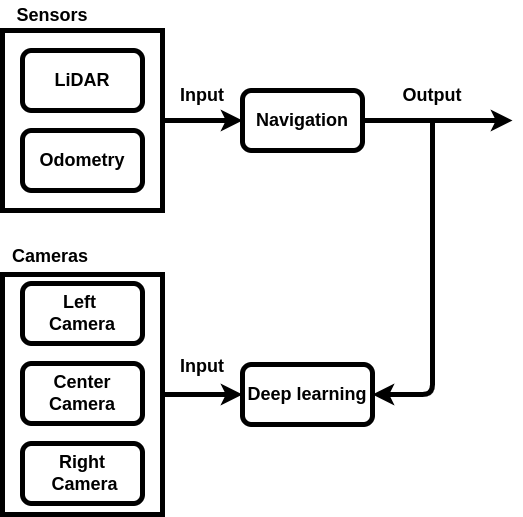
\includegraphics[scale=0.3]{images/old-method1.png}
    \subcaption{Learning phase}
  \end{minipage}
  \begin{minipage}[b]{0.45\linewidth}
    \centering
    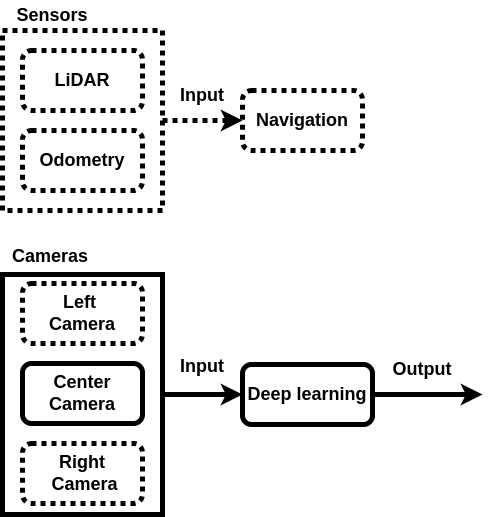
\includegraphics[scale=0.3]{images/old-method2.png}
    \subcaption{Test phase}
  \end{minipage}
  \caption{Conventional method system}
  \label{Fig:conv-method}%\vspace*{-2mm}
\end{figure}

\begin{figure}[h]
  \centering
  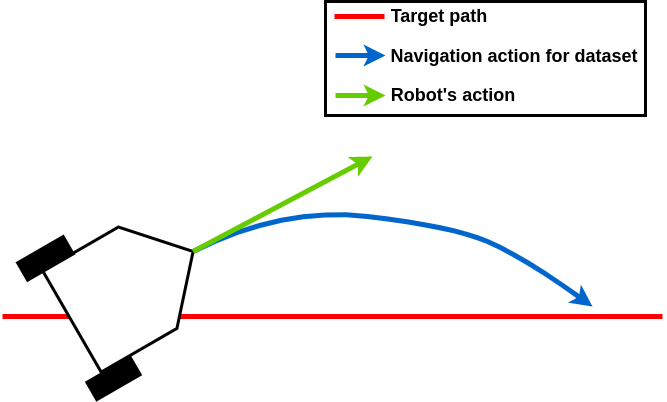
\includegraphics[keepaspectratio, scale=0.4]{images/old-method3.png}
  \caption{The conventional method collects the navigation actions apart from the robot's actions from \cite{okada-si2020}}
  \label{Fig:old-method3}
  \end{figure}

\newpage
\section{従来手法のシステム概要}
次に, 3.1章を基に構築された従来手法のシステムを\figref{Fig:okada-method}に示す. システムでは, LiDAR, オドメトリを入力としたナビゲーションの出力である角速度を学習器とモータ駆動系に与える. ナビゲーションの角速度は, ROSのパッケージであるnavigation\cite{navigation}により計算される. また, 学習器には, カメラ画像を64×48にリサイズした画像を入力し, ナビゲーションの角速度を出力して, 0.2sの周期でend-to-end学習する. 

\vspace{10mm}
\begin{figure}[h]
  \centering
  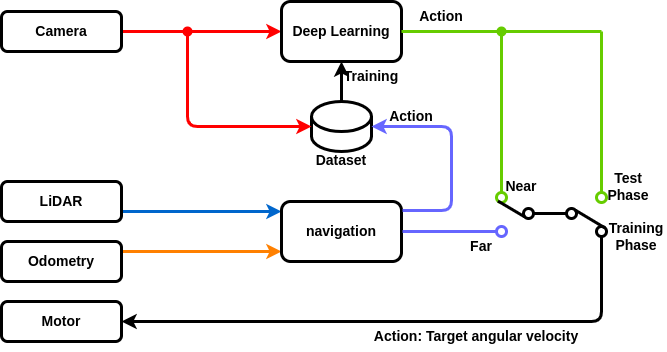
\includegraphics[keepaspectratio, scale=0.45]
  {images/okada-method.png}
  \caption{Systems that imitation learning for map-based navigation from \cite{okada-si2021}}
  \label{Fig:okada-method}
  \end{figure}

\newpage
\section{ネットワークの構造}
\figref{Fig:cnn}に従来研究で用いたネットワークの構造を示す. 構造は, 入力層1, 畳み込み層3, 全結合層2, 出力層1の計7層から構成されている.

\begin{figure}[h]
  \centering
  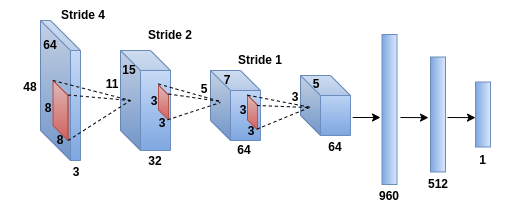
\includegraphics[keepaspectratio, scale=0.6]{images/cnn.png}
  \caption{Structure of network}
  \label{Fig:cnn}
  \end{figure}

\vspace{10mm}
従来研究ではオンラインでデータを収集し学習を行っていた. しかし, 学習器の出力で自律走行をするためには, 何周もロボットを走行させて学習する必要がある. これでは, 走行中にコースアウトしないか監視する必要や, 時間がかかるといった問題点がある. \par これらを踏まえて, 本研究では, オフラインでデータセットを収集して訓練する手法を試みる. 

